% !TeX root = ../../../main.tex
\begin{figure}[t!]

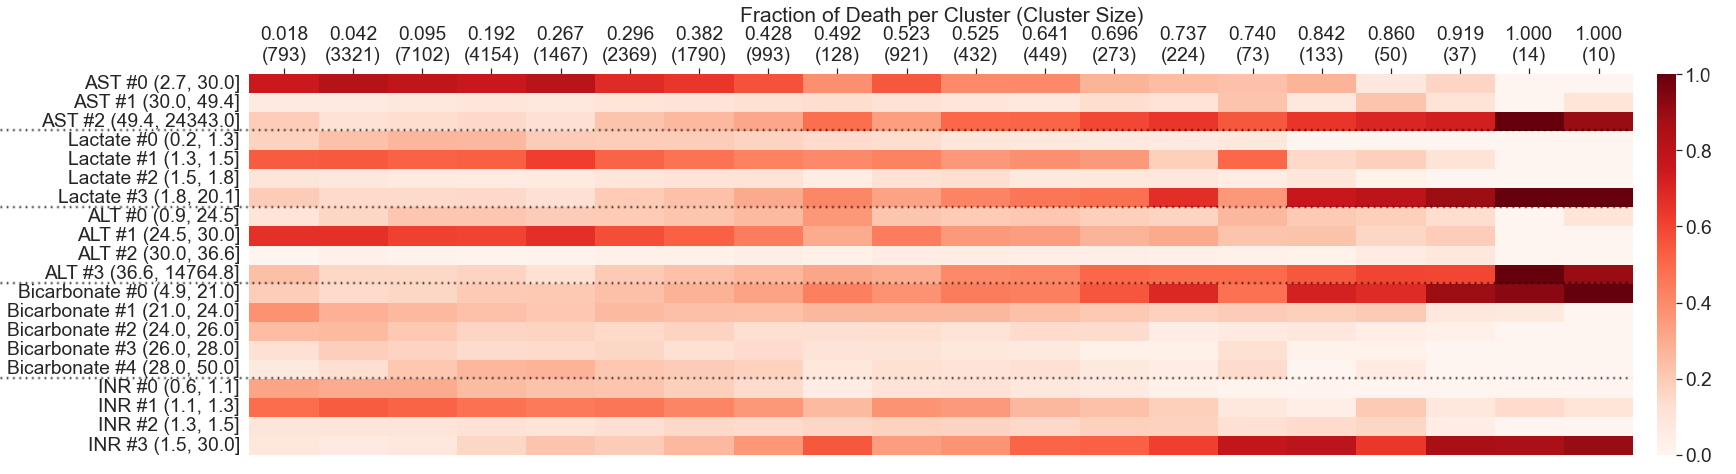
\includegraphics[width=1\linewidth]{Chapters/chapter-02/images/mimicHeatmap.png}

 \caption{Heatmap showing how features (rows) vary across clusters (columns) for the sepsis cohort of the MIMIC dataset. Heatmap intensity values can be thought of as the conditional probability of seeing a feature value (row) conditioned on being in a cluster (column); these probabilities are estimated using test set snapshots. Columns are ordered left to right in increasing fraction of test set snapshots that come from a time series that has a final outcome of death.
 }   \ChTwoFloatLabel{ch02:fig:heatmapMIMIC}
\end{figure}